\documentclass{standalone}
\usepackage{graphicx}	
\usepackage{amssymb, amsmath}
\usepackage{color}

\usepackage{tikz}
\usetikzlibrary{calc, arrows.meta}
\usepackage{pgfmath}

\definecolor{light}{RGB}{220, 188, 188}
\definecolor{mid}{RGB}{185, 124, 124}
\definecolor{dark}{RGB}{143, 39, 39}
\definecolor{highlight}{RGB}{180, 31, 180}
\definecolor{gray10}{gray}{0.1}
\definecolor{gray20}{gray}{0.2}
\definecolor{gray30}{gray}{0.3}
\definecolor{gray40}{gray}{0.4}
\definecolor{gray60}{gray}{0.6}
\definecolor{gray70}{gray}{0.7}
\definecolor{gray80}{gray}{0.8}
\definecolor{gray90}{gray}{0.9}
\definecolor{gray95}{gray}{0.95}

\newcommand*{\offset}{0.025}

\begin{document}

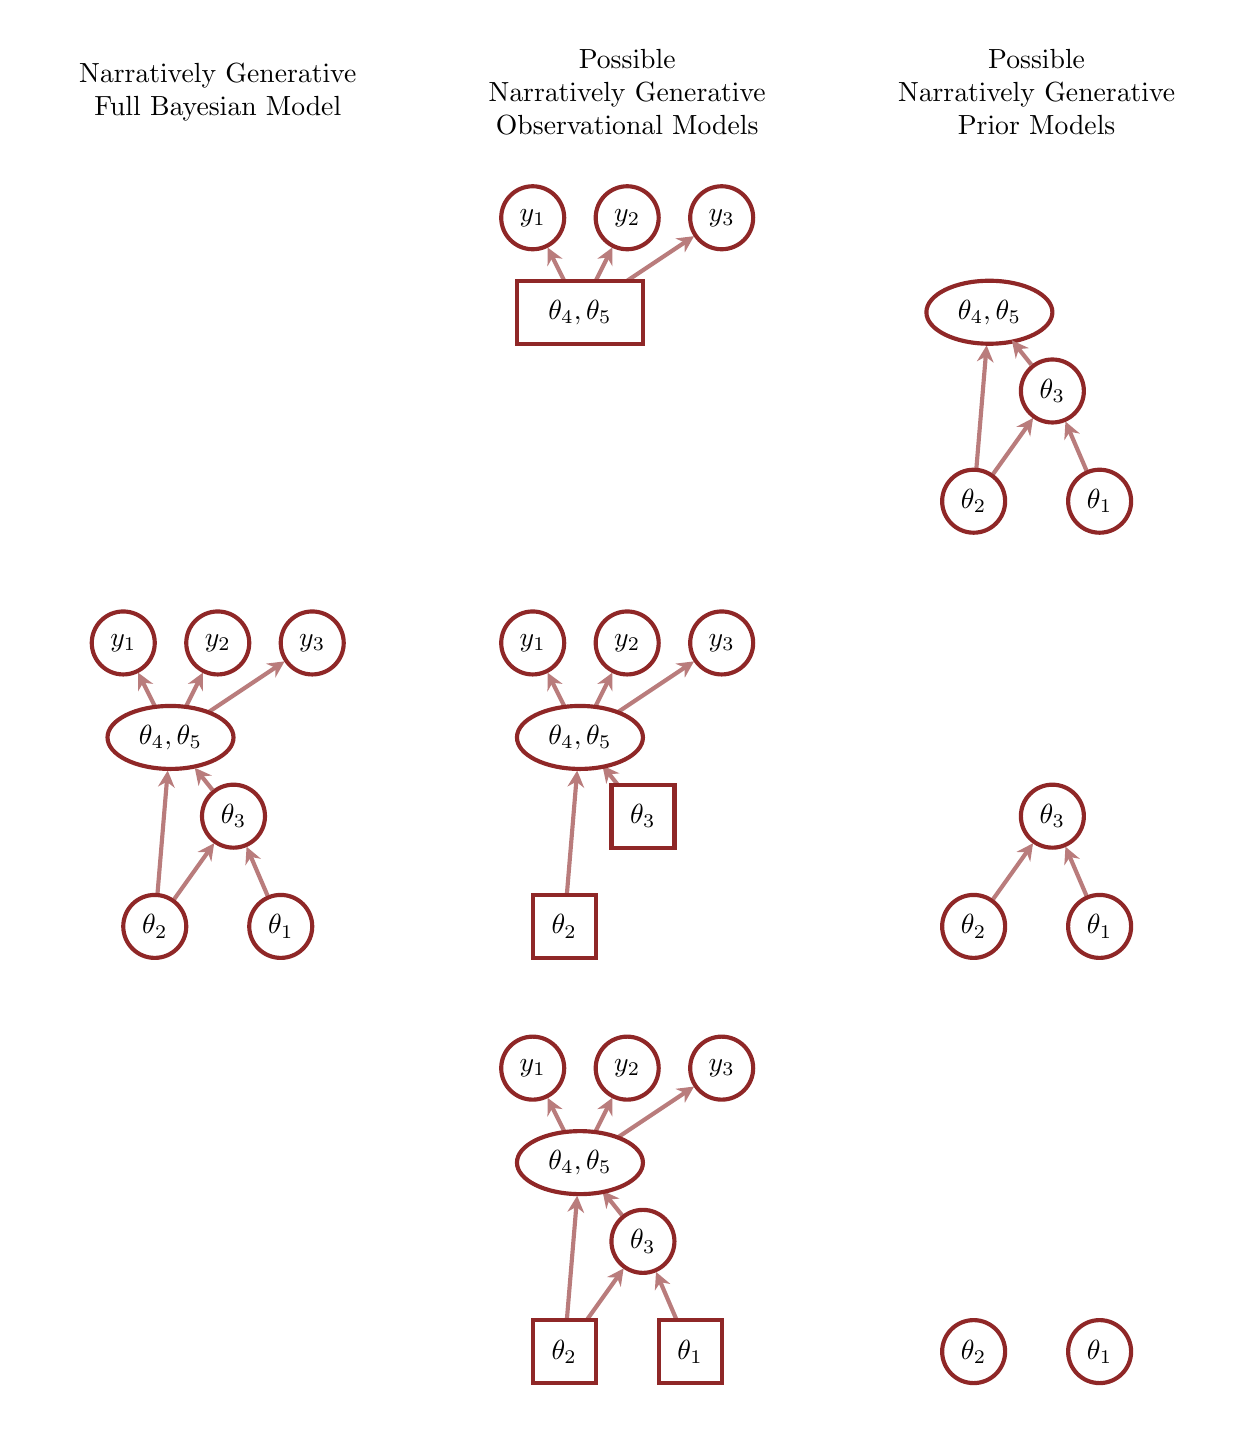
\begin{tikzpicture}[scale=0.2, thick]

  \pgfmathsetmacro{\r}{2}

  \node[align=center] at (-26, 38) { Narratively Generative\\Full Bayesian Model };
  \node[align=center] at (0, 38) { Possible\\Narratively Generative\\Observational Models };
  \node[align=center] at (26, 38) { Possible\\Narratively Generative\\Prior Models };
   
  \draw[white] (-38, 34) rectangle (38, 42);
   
  \begin{scope}[shift={(-26, -27)}]
    \draw[white] (-12, 8) rectangle (12, 34);
  
    \coordinate (A) at (4, 12);
    \coordinate (B) at (-4, 12);
    \coordinate (C) at (1, 19);
    \coordinate (D) at (-3, 24);
    \coordinate (E) at (-6, 30);
    \coordinate (F) at (0, 30);
    \coordinate (G) at (6, 30);

    \foreach \B/\E in {A/C, B/C, B/D, D/E, D/F, D/G} {
      \draw[-{Stealth[length=6pt, width=6pt]}, shorten <=12.1, shorten >=12, color=mid, line width=1.5] (\B) -- (\E);
    }

    \filldraw[fill=white, draw=dark, line width=1.5] (A) circle (\r)
    node[color=black] { $\theta_{1}$ };

    \filldraw[fill=white, draw=dark, line width=1.5] (B) circle (\r)
    node[color=black] { $\theta_{2}$ };
    
    \filldraw[fill=white, draw=dark, line width=1.5] (C) circle (\r)
    node[color=black] { $\theta_{3}$ };
    
    \filldraw[fill=white, draw=dark, line width=1.5] (D) circle [x radius={2 * \r}, y radius={\r}]
    node[color=black] { $\theta_{4}, \theta_{5}$ };
    
    \filldraw[fill=white, draw=dark, line width=1.5] (E) circle (\r)
    node[color=black] { $y_{1}$ };
      
    \filldraw[fill=white, draw=dark, line width=1.5] (F) circle (\r)
    node[color=black] { $y_{2}$ };

    \filldraw[fill=white, draw=dark, line width=1.5] (G) circle (\r)
    node[color=black] { $y_{3}$ };

    \foreach \B/\E in {C/D} {
      \draw[-{Stealth[length=6pt, width=6pt]}, shorten <=12.1, shorten >=14, color=mid, line width=1.5] (\B) -- (\E);
    }

  \end{scope}
  
 \begin{scope}[shift={(0, 0)}]
    \draw[white] (-12, 8) rectangle (12, 34);
  
    \coordinate (A) at (4, 12);
    \coordinate (B) at (-4, 12);
    \coordinate (C) at (1, 19);
    \coordinate (D) at (-3, 24);
    \coordinate (E) at (-6, 30);
    \coordinate (F) at (0, 30);
    \coordinate (G) at (6, 30);

    \foreach \B/\E in {D/E, D/F, D/G} {
      \draw[-{Stealth[length=6pt, width=6pt]}, shorten <=12.1, shorten >=12, color=mid, line width=1.5] (\B) -- (\E);
    }

    \coordinate (delta) at (2 * \r, \r);
    \filldraw[fill=white, draw=dark, line width=1.5, anchor=center] ($(D) - (delta)$) rectangle ($(D) + (delta)$)
      node[color=black, midway] { $\theta_{4}, \theta_{5}$ };
    
    \filldraw[fill=white, draw=dark, line width=1.5] (E) circle (\r)
    node[color=black] { $y_{1}$ };
      
    \filldraw[fill=white, draw=dark, line width=1.5] (F) circle (\r)
    node[color=black] { $y_{2}$ };

    \filldraw[fill=white, draw=dark, line width=1.5] (G) circle (\r)
    node[color=black] { $y_{3}$ };
    
  \end{scope}

  \begin{scope}[shift={(26, 0)}]
    \draw[white] (-12, 8) rectangle (12, 34);
  
    \coordinate (A) at (4, 12);
    \coordinate (B) at (-4, 12);
    \coordinate (C) at (1, 19);
    \coordinate (D) at (-3, 24);
    \coordinate (E) at (-6, 30);
    \coordinate (F) at (0, 30);
    \coordinate (G) at (6, 30);

    \foreach \B/\E in {A/C, B/C, B/D} {
      \draw[-{Stealth[length=6pt, width=6pt]}, shorten <=12.1, shorten >=12, color=mid, line width=1.5] (\B) -- (\E);
    }

    \filldraw[fill=white, draw=dark, line width=1.5] (A) circle (\r)
    node[color=black] { $\theta_{1}$ };

    \filldraw[fill=white, draw=dark, line width=1.5] (B) circle (\r)
    node[color=black] { $\theta_{2}$ };
    
    \filldraw[fill=white, draw=dark, line width=1.5] (C) circle (\r)
    node[color=black] { $\theta_{3}$ };
    
    \filldraw[fill=white, draw=dark, line width=1.5] (D) circle [x radius={2 * \r}, y radius={\r}]
    node[color=black] { $\theta_{4}, \theta_{5}$ };

    \foreach \B/\E in {C/D} {
      \draw[-{Stealth[length=6pt, width=6pt]}, shorten <=12.1, shorten >=13, color=mid, line width=1.5] (\B) -- (\E);
    }

  \end{scope}

 \begin{scope}[shift={(0, -27)}]
    \draw[white] (-12, 8) rectangle (12, 34);
  
    \coordinate (A) at (4, 12);
    \coordinate (B) at (-4, 12);
    \coordinate (C) at (1, 19);
    \coordinate (D) at (-3, 24);
    \coordinate (E) at (-6, 30);
    \coordinate (F) at (0, 30);
    \coordinate (G) at (6, 30);

    \foreach \B/\E in {B/D, D/E, D/F, D/G} {
      \draw[-{Stealth[length=6pt, width=6pt]}, shorten <=12.1, shorten >=12, color=mid, line width=1.5] (\B) -- (\E);
    }
    
    \foreach \B/\E in {C/D} {
      \draw[-{Stealth[length=6pt, width=6pt]}, shorten <=12.1, shorten >=13, color=mid, line width=1.5] (\B) -- (\E);
    }
    
    
    \filldraw[fill=white, draw=dark, line width=1.5] (D) circle [x radius={2 * \r}, y radius={\r}]
      node[color=black] { $\theta_{4}, \theta_{5}$ };
    
    \coordinate (delta) at (\r, \r);
    \filldraw[fill=white, draw=dark, line width=1.5, anchor=center] ($(B) - (delta)$) rectangle ($(B) + (delta)$)
      node[color=black, midway] { $\theta_{2}$ };
    
    \coordinate (delta) at (\r, \r);
    \filldraw[fill=white, draw=dark, line width=1.5, anchor=center] ($(C) - (delta)$) rectangle ($(C) + (delta)$)
      node[color=black, midway] { $\theta_{3}$ };
    
    \filldraw[fill=white, draw=dark, line width=1.5] (E) circle (\r)
    node[color=black] { $y_{1}$ };
      
    \filldraw[fill=white, draw=dark, line width=1.5] (F) circle (\r)
    node[color=black] { $y_{2}$ };

    \filldraw[fill=white, draw=dark, line width=1.5] (G) circle (\r)
    node[color=black] { $y_{3}$ };
    
  \end{scope}

  \begin{scope}[shift={(26, -27)}]
    \draw[white] (-12, 8) rectangle (12, 34);
  
    \coordinate (A) at (4, 12);
    \coordinate (B) at (-4, 12);
    \coordinate (C) at (1, 19);
    \coordinate (D) at (-3, 24);
    \coordinate (E) at (-6, 30);
    \coordinate (F) at (0, 30);
    \coordinate (G) at (6, 30);

    \foreach \B/\E in {A/C, B/C} {
      \draw[-{Stealth[length=6pt, width=6pt]}, shorten <=12.1, shorten >=12, color=mid, line width=1.5] (\B) -- (\E);
    }

    \filldraw[fill=white, draw=dark, line width=1.5] (A) circle (\r)
    node[color=black] { $\theta_{1}$ };

    \filldraw[fill=white, draw=dark, line width=1.5] (B) circle (\r)
    node[color=black] { $\theta_{2}$ };
    
    \filldraw[fill=white, draw=dark, line width=1.5] (C) circle (\r)
    node[color=black] { $\theta_{3}$ };

  \end{scope}
  
 \begin{scope}[shift={(0, -54)}]
    \draw[white] (-12, 8) rectangle (12, 34);
  
    \coordinate (A) at (4, 12);
    \coordinate (B) at (-4, 12);
    \coordinate (C) at (1, 19);
    \coordinate (D) at (-3, 24);
    \coordinate (E) at (-6, 30);
    \coordinate (F) at (0, 30);
    \coordinate (G) at (6, 30);

    \foreach \B/\E in {A/C, B/C, B/D, D/E, D/F, D/G} {
      \draw[-{Stealth[length=6pt, width=6pt]}, shorten <=12.1, shorten >=12, color=mid, line width=1.5] (\B) -- (\E);
    }
    
    \foreach \B/\E in {C/D} {
      \draw[-{Stealth[length=6pt, width=6pt]}, shorten <=12.1, shorten >=13, color=mid, line width=1.5] (\B) -- (\E);
    }
    
    
    \filldraw[fill=white, draw=dark, line width=1.5] (D) circle [x radius={2 * \r}, y radius={\r}]
      node[color=black] { $\theta_{4}, \theta_{5}$ };
    
    \filldraw[fill=white, draw=dark, line width=1.5] (C) circle (\r)
      node[color=black] { $\theta_{3}$ };
    
    \coordinate (delta) at (\r, \r);
    \filldraw[fill=white, draw=dark, line width=1.5, anchor=center] ($(B) - (delta)$) rectangle ($(B) + (delta)$)
      node[color=black, midway] { $\theta_{2}$ };
    
    \coordinate (delta) at (\r, \r);
    \filldraw[fill=white, draw=dark, line width=1.5, anchor=center] ($(A) - (delta)$) rectangle ($(A) + (delta)$)
      node[color=black, midway] { $\theta_{1}$ };
    
    \filldraw[fill=white, draw=dark, line width=1.5] (E) circle (\r)
      node[color=black] { $y_{1}$ };
      
    \filldraw[fill=white, draw=dark, line width=1.5] (F) circle (\r)
      node[color=black] { $y_{2}$ };

    \filldraw[fill=white, draw=dark, line width=1.5] (G) circle (\r)
      node[color=black] { $y_{3}$ };
    
  \end{scope}

  \begin{scope}[shift={(26, -54)}]
    \draw[white] (-12, 8) rectangle (12, 34);
  
    \coordinate (A) at (4, 12);
    \coordinate (B) at (-4, 12);
    \coordinate (C) at (1, 19);
    \coordinate (D) at (-3, 24);
    \coordinate (E) at (-6, 30);
    \coordinate (F) at (0, 30);
    \coordinate (G) at (6, 30);

    \filldraw[fill=white, draw=dark, line width=1.5] (A) circle (\r)
      node[color=black] { $\theta_{1}$ };

    \filldraw[fill=white, draw=dark, line width=1.5] (B) circle (\r)
      node[color=black] { $\theta_{2}$ };
    
  \end{scope}

\end{tikzpicture}

\end{document}  